\begin{document}

\section{Introduction}
This project has set out to create an AI that is able to play Texas Hold'em Poker. The goal of the AI is to make as much money as possible while playing. For this project we built a Texas Hold'em Poker game in Python and trained several AI's to play the game. We rewarded them based on how much money they earned. The more the better!

Texas Hold'em Poker can be played by 2 to 9 player each with a bank of starting money. The initial setup before any play occurs is as follows: First a "dealer" button is placed in front of a player (can be one of the players physically next to the dealer), a "big blind" button is placed in front of the player to the left of the "dealer" button player, then to the "big blind" players left is the "small blind" player which receives a "small blind" button. These buttons are just tokens showing the previously mentioned words on them. They rotate clockwise after each hand is completed. Once these buttons are placed the big blind and small blind players pay their blinds and place the chips in front of them. Blinds are a set amount of money of x and 2x value. For example small blind of \$5 and a big blind of \$10. Next the dealer deals each player two cards, one at a time starting with the player with the "big blind" button in front of them. 

Once the cards are dealt the first main round begins. This round consists of players initial decisions. Each player has 5 main choices when making a decision. One they can fold their hand and get rid of their cards. They are no longer in the hand. Two they can check if there is no bet they are required to match. Three they can bet an amount of money that is larger than the minimum bet and smaller or equal to what they have in their bank, if no other player has bet before them. Four, if another player has bet before them they can call the bet and match the bet with money from their bank. Five, they can raise the bet and add more money to the previous players bet. Once all the players have made their decisions and all decisions have been resolved and we reach the last player than needs to act the round is over. 

Starting the second round is the dealer who burns a card then deals three of the five community cards. This is referred to as the "flop". Once the three cards are shown another round of decisions are made by the players. Once all the decisions are resolved the round is over.

Starting the third round is the dealer who burns a card then deals one more community card. This is referred to as the "turn". Once the new community card is shown another round of decisions is made by the players. Once all the decisions are resolved the round is over.

Starting the fourth and final round is the dealer who burns a card then deals one more community card. This is referred to as the "river". Once the new community card is shown a final round of decisions is made by the players. Once all the decisions are resolved a winner is determined. The winner is determined by the player with the best 5 card hand. If two players have the same level of hand the one with the highest card value wins. For example if two players have straights, one player has 3,4,5,6,7 and the second player has 4,5,6,7,8 the second player would win.

Some notes, play can end sooner than the fourth round if all but one player folds. If a player wants to call or raise using all their chips its called going "all in". If a player who is all in loses and has no more money in their bank they are out of the game.

The AI in this case will have all the information about the current state of the game and make one of the previously discussed decisions. After a number of hands the AI will be judged and then the best performers are chosen for the next generation. This process will repeat until a set stopping criteria.


\section{Related Work}
Ever since computers have been around have we been pitting them against humans in all manners of games. Some famous examples are chess AI and GO AI that have defeated the worlds best humans at these games\cite{brown2017libratus}\cite{gilpin2005optimal}\cite{doi:10.1126/science.aay2400}. Poker is just another game waiting to be conquered by computers. However it presents a different type of game compared to chess and GO. The later games are perfect information games meaning that both (all) players can see the complete state of the game/board. Poker however is an imperfect information game meaning that one player can not have/see the complete state of the game/board\cite{brown2017libratus}\cite{davidson2000improved}\cite{gilpin2005optimal}\cite{gilpin2006competitive}\cite{doi:10.1126/science.aay2400}. This forces the AI to have to guess about what action to take since they do not have all the information. This has been the trickiest part of making an unbeatable poker AI. This task also applies to many real world applications that also deal with imperfect information.

In order to solve this problem many different approaches have been taken. "Libratus: The Superhuman AI for No-Limit Poker" has taken a three module approach to the problem\cite{brown2017libratus}. Libratus consists of a pre-computing module, a nested sub-game solver module and a self improvement module. The first module deals with the general strategy of the AI and makes categories of all the possible situations and actions that could be made from that point. It has two kinds of abstractions that it groups these situations into: action abstraction and card abstractions\cite{brown2017libratus}. The card abstractions deal with the possible card combos at each stage of play and lumps groups of card possibilities into buckets that millions of card combos. This is only employed on the last two rounds of play\cite{brown2017libratus}. The use of abstractions gives the AI a general game plan and one that will be refined in the second module. The abstracted game that is created in this module is solved with a distributed version of an improvement over Monte Carlo Counterfactual Regret Min-imization (MCCFR)\cite{brown2017libratus}.

The second module examines the game at a finer detailed level to make the best decision it can. Since an imperfect information game cannot be solved on its own the AI second module looks at sub games similar to the one that it is trying to solve and uses that information to make its decision\cite{brown2017libratus}. The third and final module is the self improvement model. It uses the previous data and the outcome of the most recent hand to fine tune its performance. It learns what sub games it should have used and how to arrive at that conclusion in the future\cite{brown2017libratus}.

Another approach is taken by "Poki" which is a poker AI that specifically focuses on opponent modeling\cite{davidson2000improved}. Poki's goal is to keep track of how opponents are playing, how it expects them to play and to react to these factors. Poki uses an artificial neural net to keep track of and predict its opponents actions. Poki used feed-forward and back propagation algorithms to tune the model. This model had much better results at predicting opponents actions than previous attempts\cite{davidson2000improved}.

Another approach uses "Rhode Island Hold’em Poker" to accomplish the goal of training a poker playing AI. Rhode Island Hold'em Poker is a simplified version of Texas Hold'em Poker than contains less possible states the game can be in making the imperfect information problem easier to solve\cite{gilpin2005optimal}. The goal for this approach is to train and develop models on a less complex version of the imperfect information problem so that these models can become really good at this version quicker and more efficently before being applied to the more complex problem\cite{gilpin2005optimal}.

From looking into all these different approaches we decided to combine a few and apply a neural net to a slightly simplified version of Texas Hold'em Poker. Where our focus was on the decision making of the AI to make the most money possible.

\section{Approach}
\subsection{Data/Problem Analysis}
The data in this problem is poker hands, games and the results of them. We did not use any historical data for
this solution. All data was used for the AI learning while it played the game. We valued AI that could win the
most money. NATHAN MAYBE SOMETHING HERE ABOUT THE VALUE FUNCTION??? IT COULD GO LATER

The fitness function is inside of a self\_evaluate function in NeatPlayer(Not the best place I know), and the
algorithm is as follows: 
\begin{minted}{python}
def self_evaluate(self) -> None:
    final_money = self.money
    delta_money = self.total_bets
    value_of_betting = 0.1
    fitness = 0
    if abs(delta_money) < self._start_money/10:
        #punish AI severely for not betting alot
        fitness = 0
    else:
        # reward the AI for taking larger bets too
        fitness = final_money + value_of_betting*abs(delta_money)
    return fitness
\end{minted}


\subsection{Resources Used}
Our programming language of choice is the same as the one from this class, Python 3. We used several libraries
and they can be found in the below table \autoref{tab:libs}. The most important of these is the Neat library.
The Neat library is the one that we use for the AI. The neat library is a pure python implimentation of NEAT.
IE theere there is no dependency on Tensorflow or anything(sadly). However it is a very solid library for NEAT,
allowing alot of customizaiton from mutation rates and strengths, to starting network topology, activation
functions and more!

\begin{table}[H]
    \caption{Python Libraries Used}
    \centering
    \begin{tabular}{ | l |}
    \hline
        Library name \\
        \hline
        \hline
        numpy \\
        itertools \\
        tensorflow.keras \\
        neat \\
        logging \\
        pytest \\
        functools \\
        graphvis \\
        warnings \\
        matplotlib.pyplot \\
        os \\
        copy \\
        
    \hline
    \end{tabular}
    \label{tab:libs}
\end{table}

\subsection{Software Design}
Our software design was a bottom up object oriented design. There is two halves to solution. One half is the poker game itself and the second half is the AI that can play the poker game. The first half, the poker game was built bottom up objected oriented starting with the basic building blocks of the poker game. First a card was implemented then a deck. From there the logic of the game was implemented in pieces where each piece added more complexity. Pieces include, players, hands, community cards, board, hand values, rounds and games etc. 

Once the game was complete the next step was adding the Neat integration to create the AI player. For the AI
the first step was to get a basic set up of the AI, and to do this we used a NEATPlayer which is a player that
holds a neat algorithm for playing. This player is used in order to interact the the Board(which as a reminder
manages the game).

In main.py and config-feedforward the configuration can be seen for the Neural networks, first we used the ReLU
activation to encourage big bets, and we dont care about negative bets(and we wanted a system that can handle
non-linear system as poker is 100\% not linear). The mutation rates are all set to 0.2, as this was a decent
number that allowed for some mutation but not so high that innovations are lost.
The system is also designed to start with 10 hidden nodes, these are dense nodes that allow the system to have
some compexity starting out to give it a chance to do something, but this model is quickly dropped as can be
seen in some of the images. The Neural network has 74 inputs, which is alot for a small network, and this
information ranges from the pot, to the public cards, and a variety of other factors. This is also still a
simplification of both the rules and the information of poker and there are multiple featuers that are just not implimented.
S
In this algorithm you can see the AI is rewarded not only for winning money, but also for placing more bets
down. This is due to the fact that one of the earlier problems occured in training was the AI would learn the
best way to win was to just not bet at all and just hoard thier money. As a result, if the AI does not bet
enough money it is automatically given a score of 0. However to encourage the AI to not just sneak in with betting just over the limit, I reward the AI for any bets it makes(and then if it wins money it obviously gets more
money). This fixed the issue(along with some other fixes).

At the top of the config file you can see the population size as 5000, which is a good critical mass of players
to make sure that learning actually occurs. The threshold is just some stupid high number to make sure that the
main.py goes through all of the generations, it is irrelvient.

The number of generations is set in the main.py, and it typically ranges between 100-1000 for most testing.
Ideally this would be much higher as NEAT can take while to get off of the ground however these tests are being
run on my laptop during pre-finals time.... so the available computer time is limited.

Finally, a large emphasis was placed on implimented Test Driven Development in order
to create more reliable software that we know is working as intended. This was especially important for writing
the rules of Poker which are complex and ensuring the intended behavoir was correctly implimented can be
incredibly time consuming. As a result of this, we implimented a Test Suite with pytest. All tests for the
codebase can be run by using the pytest command in the terminal at the root of the project.
\begin{minted}{bash}
 $ pytest
\end{minted}

This allows the team to be confident that the software written is correct and new additions do not
unintentionall break older changes, giving the team greater development throughput especially towards the end
of the project

\clearpage
% THIS WILL HAVER TO BE PLAYED WITH
\begin{figure}[H]
    \centering
    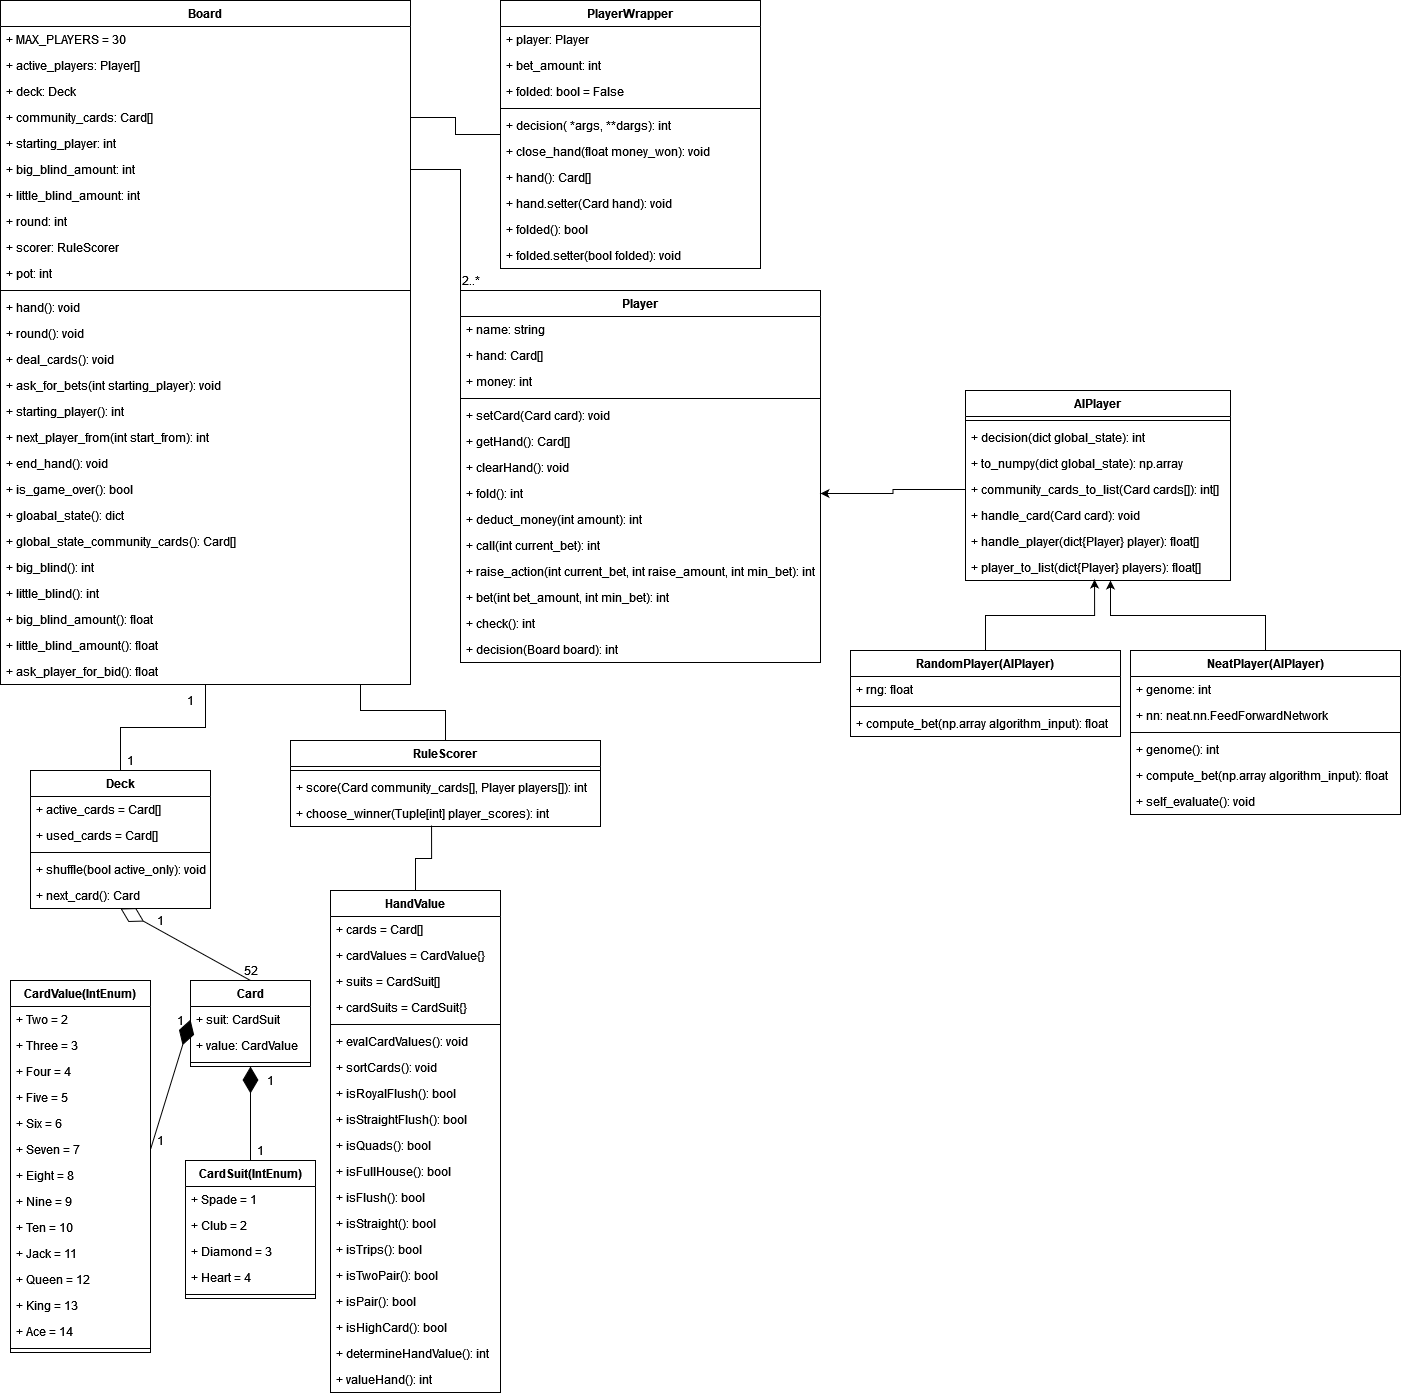
\includegraphics[scale=0.4]{resources/Poker_AI_-Class_Diagram.drawio.png}
    \caption{Class Diagram for our Poker AI}
    \label{fig:classDiagram}
\end{figure}
% \image{resources/Poker_AI_-Class_Diagram.drawio.png}{Class Diagram for our poker AI}{fig:classDiagram}



\subsection{Source Code Description}
\begin{table}[H]
    \caption{Source Code Files}
    \centering
    \begin{tabular}{ | c | p{14cm} |}
    \hline
         File Name & Description \\
        \hline
        \hline
        main.py & The driver of the program\\ \hline
        visualize.py & Creates the graphs and visuals\\ \hline
        AIPlayer.py & Implements AI Player class both random and Neat player\\ \hline
        Board.py & Poker board (table) implementation. All the control logic for how the game is played is handled here\\ \hline
        Card.py & A playing card implementation\\ \hline
        Deck.py & Deck of Cards implementation\\ \hline
        HandValue.py & Evaluator for hands value. Uses the official poker ranking for determining hand value\\ \hline
        Player.py & Poker Player functionality. Fold, check, bet, raise, call, cards in hand and money\\
        Mock\_player.py & \\ \hline
        test\_AIPlayer.py & Test cases for the AIPlayer Class \\ \hline
        test\_Board.py & Test cases for the Board Class\\ \hline
        test\_Card.py & Test cases for the Card Class\\ \hline
        test\_Deck.py & Test cases for the Deck Class\\ \hline
        test\_HandValue.py & Test cases for the HandValue Class\\
        
    \hline
    \end{tabular}
    \label{tab:sourceCode}
\end{table}

\section{Evaluation and Results}

\subsection{Results}
There are two important graphs that come out of training in order to determine how the system performed over
time. These are: the fitness over generations, which plots the fitness score over time, then there is the
generation comparison which plots the results of a generation comparison game that is played at the end of
training. THe reason for this second graph is two-fold: first, it allows a direct comparison between the various
models to be done to show any learning over time, second it allows us to verify the fitness function is
producing the desired results because as was discussed in the software architecture there were issues with the
fitness function encouraging the AI's to not bet. Howver this means that the fitness function is not the true
metric we were really looking for and as a result, we wanted to check the final output to make sure the AI was
still winning.

\image{resources/generation_comparison.png}{Generation Comparison}{fig:genComp}
\image{resources/Fitness_over_time.png}{Fitness over the generations}{fig:fitness}


\subsection{Results Discussion}
As can be seen in the graph, in the \autoref{fig:fitness} the earlier models seem to be much better than the
final models as thier fitness is much higher, however it is important to note that in poker, the fitness
score is relative to the other players, meaning that at the start, when players are random and some are just by
chance by chance better or luckier there is a good chance of players being able to just steal other-players out
of money, resulting in not only high bets but also lots of money won.

However over time as the general population becomes not terrible at poker, the overall fitness goes down. This
hypothesis is also shown in the generation comparison, as the initial AI, despite having a very high score,
performs very poorly against later versions as it was likely a combination of luck and per performance of the
other models that allowed the early models to succeed.

You will also note that the generation limit and population sizes are rather low for a NEAT algorithm, which
causes a signifcantly lower learning rate as NEAT usually needs a critical mass of players in order for learning
to occur, This is down to a few factors discussed below.

The first issue is limitations in computation time, as this analysis was mostly performed in the pre-finals time
on a team-members laptop, which meant laptop-time was in high demand. In attemps to optimize the codebase in
order to run higher populations and more generations in less time, we ran into the issue of the python-NEAT
library hitting hard performance limits, as it was not meant for a game as complex as poker in such a confined
time environment, and despite the fact that the poker game could run 100s of batches with 1000s of players in
less than a second, the neat-AI library would then take a minute or two to perform mutations and other
necessary functions for that generations, which essentially put a cap on the size of the population that could
be performed.

One graph not shown as it turned out to not be relevant was the performance of the AI against a random player,
this is because even by generation 5 with a small-ish population, the Neat-AI absolutely robs that player of all
of thier money and causes them to lose, so the graph was two horizontal lines, one with the neat-ai player
that had all the money, and one with the random player with no money

\section{Conclusion}
In conclusion, the overall model performed decently and with more computer time, and a more optimized
NEAT library, NEAT stands a chance of performing optimally for an unknown complex game like poker. 



\section{References}
\printbibliography

\section{Appendix: Personal Contribution and Lessons Learned}
\subsection{JP}
My personal contributions were to the brainstorming and deciding on the topic for the project, helping design the implementation of Texas Hold'em Poker in Python 3, creating and formatting the presentation, creating and the initial formatting of the final report. Writing the introduction, related works, a portion of the approach section, created the class diagram, creating the file description table, compiling the libraries used table. For the implementation I specifically wrote the hand value and player classes for the Texas Hold'em Poker Game as well as the tests for these class.

For lessons learned. I learned that the power and capabilities of a poker playing AI is really interesting and hard to get a complete one working. I discovered this while reading all the previous research and seeing how far they have come but also how far they have to go. The idea of an imperfection information problem is nothing new to humans and I believe we are uniquely suited for that kind of problem but computers are not. They are designed for complete information problems. When dealing with incomplete information problems with computers is where the human inspired neural networks come into play and they have had the most success in these problems. Early computers were just not powerful enough. So knowing where they came from to see Nathan and I be able to create pretty decent Texas Hold'em AI players is pretty neat (pun intended). Although we used a slightly simplified version it is still really rewarding to see the outcome. 

One thing I did not expect was that during our training and testing of the models there was original one AI just completely destroyed the random AI. I would have expected it to take a while to learn a decently complex game. From this we put several AI players against each other instead of having the random AI and it improved all the AI players. It was really interesting to see the growth of the best AI model over generations of its development. Some times it was really clear who the best was and sometimes it was back and forth or sometimes the AI would regress in skill, which I did not think it would do.
\subsection{Nathan}
My contribution was as the primary coder, JP came up with the idea and scoped the project, and then I created
the structure and coded some of the more complex areas of the code. Also I was the primary person responsible
for integrating NEAT into Poker and ran the tests on my laptop. Tweaking of the Neural network was performed
by me with help from JP. Then of course I assisted JP with the final documentation.

Lessons As for lessons learned, I now have a new respect for competitive unsupervised learning, as it is
difficult to rate how well you are becoming in a game like poker as in addition to the game just being complex,
there is ALOT of chance involved that prevents accurate fitness functions. In addition the fact that the score
is based on the other players performance not just the AI's own performance makes it a non-ideal fitness
function, however for a game like Poker we were unable to come up with a better metric.

In addition we had the idea that we could compare the initial learning against a random AI, but that turned out
to not work very well at all, as even by generation 5, NEAT absolutey destroys the randomAI ruining our initial
performance graphs ideas. So I guess the lesson learned from this is: always make sure you come up with multiple
methods of measuring performnace


\end{document}